\documentclass{article}

\usepackage{amsmath}
\usepackage{amssymb}
\usepackage{amsxtra}
\usepackage{graphicx}
\usepackage{listings}
\usepackage{subcaption}
\usepackage[margin=1.2in]{geometry}

\newcommand{\refchapter}[1]{Chapter~\ref{#1}}
\newcommand{\refsec}[1]{Section~\ref{#1}}
\newcommand{\refeqn}[1]{Equation~(\ref{#1})}
\newcommand{\reffig}[1]{Figure~\ref{#1}}

\title{\bf Software Lab \\ Computational Engineering Science \\
{\Large Pusher Mechanism}} 

\vspace{1.5cm}

\author{Aaron Albert Floerke, Arseniy Kholod, Xinyang Song, Yanliang Zhu \\[1cm]Supervisor: Dr. rer. nat. Markus Towara\footnote{Informatik 12: Software and Tools for Computational Engineering, RWTH Aachen University, {\tt info@stce.rwth-aachen.de}}}


\date{{\begin{center} 18\textsuperscript{th} November 2024 \end{center}} 
\includegraphics[width=.6\textwidth]{rwth_i12_softw-werkz_en_rgb}}

\begin{document}

\lstloadlanguages{Python}
\lstset{basicstyle=\small, numbers=left, numberstyle=\footnotesize,
  stepnumber=1, numbersep=5pt, breaklines=true, escapeinside={/*@}{@*/}}

\pagestyle{plain}

\maketitle

\clearpage

\tableofcontents

\clearpage

\section*{Preface}

The topic "Pusher Mechanism" was assigned as a final project by the Department of Informatik 12: Software and Tools for Computational Engineering, RWTH Aachen University, for the Software Lab course in the Computational Engineering Science B.Sc. program. This work was carried out under the supervision of Dr. rer. nat. Markus Towara.

This project involves developing an enhanced version of the well-known planar four-bar linkage, a mechanical system widely used in applications like conveyor systems, oil well pumps, and robotic arms. By adding an extra joint, the extended mechanism offers more degrees of freedom, making it better suited for specific tasks. In this work, we designed and implemented this extended four-bar linkage to find a suitable mechanism for moving a box along a conveyor while avoiding obstacles.

In the first phase of the project, we analyzed the user requirements provided by our supervisor and broke them down into system requirements. This was followed by a theoretical analysis of the mechanism's geometry. Based on this analysis, we selected Python as the implementation environment due to its suitability for the task and the team's expertise.

The implementation consists of three interconnected components. First, the backend was developed to handle the geometry of the linkage, calculating the coordinates of all joints based on input parameters to ensure accurate modeling.

The second component is the frontend, a graphical user interface (GUI) created with the Tkinter\footnote{https://docs.python.org/3/library/tkinter.html} library. It enables users to visualize the linkage’s movement, modify its parameters, and display essential information about the mechanism.

Additionally, a well-documented testing process was carried out to ensure the correctness and reliability of both the backend and frontend. This testing verified the system's performance across various scenarios, ensuring its accuracy and robustness.

With our implementation, we successfully addressed the optimization problem of moving a box along a conveyor while avoiding obstacles. The addition of an extra joint to the four-bar linkage provided the necessary degrees of freedom, enabling precise trajectory design. This solution met the system and user requirements and demonstrated the mechanism's effectiveness in achieving task-specific motion.

Furthermore, detailed documentation of the software and project management processes was created to enhance maintainability and offer a clear understanding of the project’s structure. This documentation ensures that future developers or users can efficiently modify and extend the system. Overall, this work demonstrates the successful combination of theoretical analysis, design, and practical implementation in creating a functional pusher mechanism.

\clearpage

\section{Introduction}

The industrial revolution in the 18th and 19th centuries brought about significant advancements in manufacturing processes, one of which was the challenge of transporting products efficiently between various workstations in factories. A key solution to this challenge was the development of mechanical systems like the four-bar linkage, which can be used as a pusher mechanism to move products along production lines or between different conveyor systems. Despite its simple structure, the four-bar linkage has proven to be an effective mechanism in various industrial applications. 

Over time, the four-bar linkage model has expanded beyond basic conveyor systems and has found applications in more complex systems, such as pumpjacks, robotic arms, and automotive engineering. Its simplicity and efficiency continue to make it relevant in modern mechanical design.

In this work, we aim to analyze the theoretical principles behind the four-bar linkage, design and implement an extended version of the mechanism with an additional joint, named coupler (see Figures \ref{fig:linkage-1} and \ref{fig:linkage-2}), and apply it to solve the problem of moving a box along a production line while avoiding obstacles. By enhancing the classic four-bar linkage, we seek to provide a more flexible solution suited to complex real-world tasks.

\begin{figure}[h]
	\centering
	\begin{subfigure}{0.49\textwidth}
		\centering
	    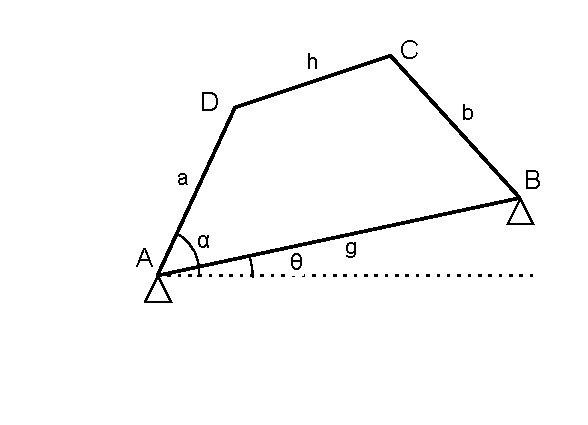
\includegraphics[width=\linewidth]{./figures/four-bar_linkage.pdf}
	    \caption{Planar four-bar linkage}
	    \label{fig:linkage-1}
	\end{subfigure}
	\hfill
	\begin{subfigure}{0.49\textwidth}
		\centering
		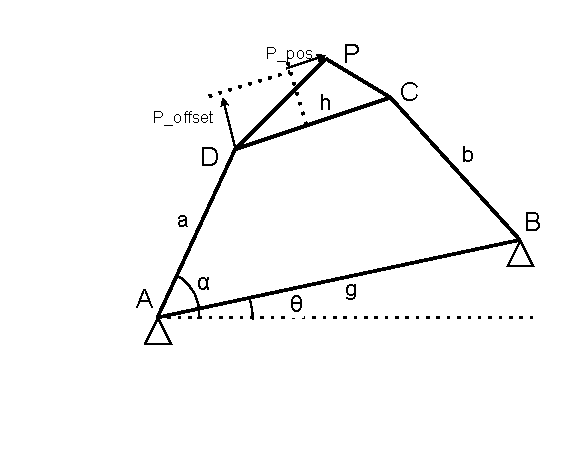
\includegraphics[width=\linewidth]{./figures/four-bar_linkage+coupler.pdf}
		\caption{Planar four-bar linkage with coupler P}
		\label{fig:linkage-2}
	\end{subfigure}
	\caption{Four-bar linkage}
\end{figure}

The structure of this paper is as follows: In Section \ref{ch:analysis}, we analyze the user requirements, derive the system requirements, and provide an overview of the theoretical analysis of the mechanism’s geometry. Section \ref{ch:design} covers the selection of the implementation environment, taking into account the system requirements and the team's expertise, as well as the preparation of UML class models for the implementation phase. Section \ref{ch:implementation} describes the implementation of the four-bar linkage, the graphical user interface, and the software testing process, while Section \ref{ch:doc} provides software documentation to ensure its maintainability. In Section \ref{ch:optimization-problem}, we use the developed software to determine the appropriate mechanism parameters to move the box along the conveyor. Finally, in Sections \ref{ch:projectmanagement}, we discuss our project management.

\section{Analysis} \label{ch:analysis}

\subsection{User Requirements}

\begin{figure}[h]
	\centering
	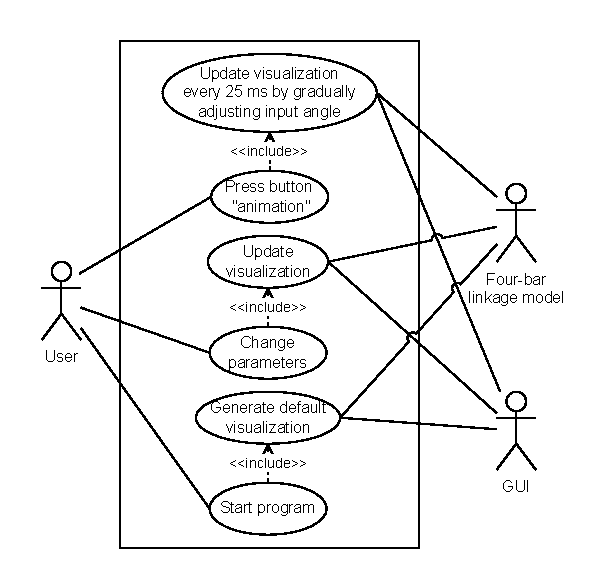
\includegraphics[width=0.7\textwidth]{./figures/uml_use_case.pdf}
	\caption{UML use case diagram}
	\label{fig:use_case}
\end{figure}

User requirements outline the overall vision for how a system should function and what features it must provide to meet user needs. These high-level expectations are the foundation for developers to derive more detailed and technical system requirements, which define constraints and specifications the software must fulfill.

To enhance understanding of the user requirements described later, we provide a UML use case diagram of user-software interactions in Figure \ref{fig:use_case}. The diagram illustrates the main workflow: after starting the program, the user is presented with a default visualization of the four-bar linkage generated by the GUI and the linkage model. The user can modify this visualization by specifying input parameters through the GUI. Additionally, the four-bar linkage can be animated, with the input angle gradually increasing and the visualization updating every 25 ms upon the user’s explicit request.

The following list presents all the user requirements provided by our supervisor, along with our explanations and interpretations of each concept.

\begin{itemize}
	\item \textit{Requirement: Implement all motion types of a planar four-bar linkage extended with a coupler.}
	
	The planar four-bar linkage extended with a coupler, illustrated in Figure \ref{fig:linkage-2}, may appear to be a straightforward geometric structure. However, its motion is more complex than it seems. While the coupler $P$ does not influence the primary motion constraints, the lengths of the four main bars define the limitations of the input angle $\alpha$. These constraints can result in the input angle being unlimited, symmetrically limited, or asymmetrically limited relative to the ground link $AB$. Consequently, the links $AD$ and $BC$ can function as either cranks, capable of full rotation, or rockers, which only partially rotate. In fact, as explained in \cite{inproceedings}, 27 distinct motion types for such mechanisms have been identified. A deeper analysis of these motion types will be conducted in the theoretical section of our study.
	
	\item \textit{Requirement: Implement a graphical user interface (GUI) to display four-bar linkage animation and customize its geometric parameters.}
	
	The GUI should enable users to visualize the linkage, provide smooth animations, and adjust various geometric parameters of the system. We have identified eight key parameters (degrees of freedom) that the GUI should support:
	\begin{itemize}
		\item The lengths of the four bars ($AB$, $BC$, $CD$, $AD$).
		\item The angle $\theta$ between the fixed bar $AB$ and the horizontal line.
		\item The input angle $\alpha$ between the bar $AD$ and the horizontal line.
		\item The position of the coupler relative to the middle of the floating link, expressed by $P_{pos}$ and $P_{offset}$.
	\end{itemize}
	During the animation process, the input angle $\alpha$ is no longer a free parameter, as it is dynamically determined by the system to ensure smooth motion.
	
	Additionally, while the position of point $A$ could be considered an independent parameter (technically two parameters in 2D), for simplicity, we assume it is fixed at $(0, 0)$ during geometric analysis. If point $A$ needs to be positioned elsewhere, the entire linkage can simply be translated accordingly. This fixed-point assumption will simplify the design phase but can be revisited for solving optimization problems later.
	
	\item Find and provide suitable parameters for the pusher mechanism to meet requirements of the following optimization problem:
	\begin{itemize}
		\item Push box with size $80\times60$ from $x=220$ to $x=0$
		\item Do not cross the area of the labeling machine (Area with $x<80$ and $y>70$).
		\item Pass above points $(120, 80)$ and $(220, 80)$
	\end{itemize}
\end{itemize}

\subsection{System Requirements}
Functional
\begin{itemize}
	\item \textbf{Four-bar linkage model}:
	\begin{itemize}
		\item System simulates all 27 motion types of the four-bar linkage with coupler.
		\item System does not crash with any parameter input.
		\item System validates input data.
	\end{itemize}
	\item \textbf{Tests}:
	\begin{itemize}
		\item Implement test cases to cover all motion cases.
		\item Provide reference data to compare results with.
	\end{itemize}
	\item \textbf{Graphical User Interface}:
	\begin{itemize}
		\item GUI is coupled with the four-bar linkage model to use implemented motion cases for animation. 
		\item GUI provides the four-bar linkage visualization.
		\item GUI has slide bars to input geometrical data.
		\item GUI reacts to new input data by changing the four-bar linkage visualization accordingly.
		\item GUI provides animation of the four-bar linkage motion.
		\item GUI provides tracing of the coupler to show its trajectory.
	\end{itemize}
	\item \textbf{Optimization problem}:
	\begin{itemize}
		\item GUI visualizes the solution.
	\end{itemize}
\end{itemize}
Non-functional
\begin{itemize}
	\item \textbf{Performance}:
	\begin{itemize}
		\item The four-bar linkage model is fast enough to provide smooth GUI animations.
		\item GUI animations are not slower than 30 frames per second.
	\end{itemize}
	\item \textbf{Usability}:
	\begin{itemize}
		\item GUI and four bar linkage implementation are well-documented.
	\end{itemize}
\end{itemize}

\subsection{Theory}

explain geometry

\section{Design} \label{ch:design}

\subsection{Principal Components and Third-Party Software}

libraries that you built on explained briefly and references to further information

\subsection{Class Models}

UML Class diagram(s) and description; should link into overall design through
reference of application programming interfaces (API) of third-party software

\section{Implementation} \label{ch:implementation}

\subsection{Development Infrastructure}

programming language, compiler, run time libraries, target platform
(hardware, operating system)

\subsection{Source Code}

overview of source code structure (file names, directories); build instructions; references into source code documentation e.g, doxygen\footnote{\tt https://github.com/doxygen/doxygen}; short (!) code listings
\begin{lstlisting}
#include<iostream>
int main() {
  std::cout << "Leave me alone world!" << std::endl;
  return 42;
}
\end{lstlisting}
if helpful (must come with detailed explanation)

\subsection{Software Tests}

e.g, googletest\footnote{\tt https://github.com/google/googletest}

\section{Documentation}\label{ch:doc}

\section{Optimization Problem}\label{ch:optimization-problem}


\section{Project Management} \label{ch:projectmanagement}

who did what, when, and why; organization of collaboration, i.e. [online] meetings, software version control (e.g, git\footnote{\tt https://git.rwth-aachen.de}

\bibliographystyle{plain}
\bibliography{literature}

\appendix

\section{User Documentation} \label{ch:userdoc}

\subsection{Building}

e.g, using cmake\footnote{\tt https://cmake.org/} and make\footnote{\tt https://www.gnu.org/software/make/}


\subsection{Testing}

e.g, \verb!make test!

\subsection{Running}

documented sample session(s); e.g, \verb!make run!


\end{document}

